\chapter{Project documents}
Here documents produced in relation to the project will be presented. Both status reports and activity plans were to be created and delivered to the supervisor every other week. 

\section{Status report example}
%Tried to make it look as much as the actual status report as possible. That's why it looks a bit funny.
Below is a copy of an status report made by the group for the supervisor. This status report is for the weeks 6 and 7.\\
\newline

\textbf{1. Introduction}\\
These two weeks were the first weeks of project work, since little could be done prior to meeting the customer. During the first week there was one member missing.\\
\newline

\textbf{2. Progress summary}\\
In this two-week period we have completed on average 68\% of the work scheduled on the activity plan. We believe that we still are on schedule according to the milestones set by the customer. The work that was done was in general related to the design of the final product and making sure we have all the required libraries, licenses and other factors that need to be in order before we start programming the actual product.\\
\newline

\textbf{3. Open / closed problems}\\
\newline
\textbf{Open:}
\begin{itemize}
	\item{New requirements: friendlier bluetooth device pairing}
	\item{Bluetooth connection: need a bluetooth module to the arduino}
	\item{Not documented preexisting code}
	\item{Decide on a product name}
\end{itemize}
\vspace{8mm}

\textbf{Closed:}
\begin{itemize}
	\item{Lacking source code: Will not use the compiled program in question}
	\item{Licenses: separate out licensed components into separate projects}
\end{itemize}
\vspace{8mm}

\textbf{4. Planned work for next period}\\
For next period we will have to complete the designs of the project and complete version 0.1 to show to the customer.\\
\newline

\textbf{5. Updated risks analysis}\\
\begin{itemize}
	\item{License incompatibility: impact has gone down from 8 to 7. Importance has gone down from 10 to 8. This is because of information from the customer about ways to circumvent this issue (as mentioned above).}
\end{itemize}

\section{Activity plan example}
Below is an example of an activity plan made by the group for the supervisor. This activity plan is for the weeks 6 and 7.\\

\begin{figure}[H]
\makebox[\textwidth][c]{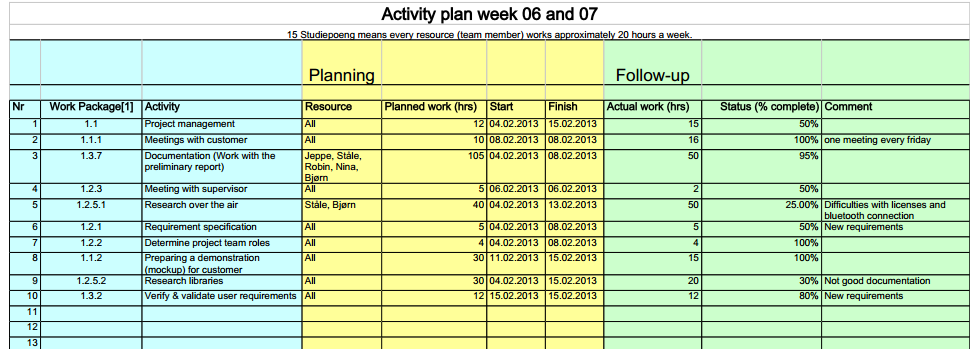
\includegraphics[width=1.3\textwidth]{images/activity_plan_example.png}}
\caption{Example activity plan for the weeks 6 and 7}
\end{figure}
